% Chapitre 2 : Théorème de Pythagore et sa réciproque
% Version améliorée conforme à la réforme du collège 2025
\chapter{Théorème de Pythagore et sa réciproque}

\section{Introduction}
Le théorème de Pythagore est l'un des théorèmes les plus célèbres et les plus utiles de la géométrie. Il porte le nom de Pythagore, mathématicien et philosophe grec du VI\textsuperscript{e} siècle avant J.-C., bien que cette relation ait été découverte par plusieurs civilisations antérieures (Babyloniens, Égyptiens, Chinois).

Ce théorème établit une relation fondamentale entre les côtés d'un triangle rectangle et trouve de nombreuses applications dans la vie courante : architecture, navigation, cartographie, sport, etc.

\textbf{Problématique du chapitre :} Comment calculer des longueurs dans un triangle rectangle ? Comment déterminer si un triangle est rectangle ?

\section{Activité d'approche : découverte par manipulation}

\textbf{Objectif :} Découvrir la relation entre les aires des carrés construits sur les côtés d'un triangle rectangle.

\textbf{Matériel :} Papier quadrillé, ciseaux, règle graduée

\textbf{Consigne :}
\begin{enumerate}
    \item Construire plusieurs triangles rectangles sur papier quadrillé
    \item Construire un carré sur chacun des trois côtés
    \item Compter le nombre de carreaux de chaque carré
    \item Chercher une relation entre ces trois nombres
\end{enumerate}

\textbf{Constat :} Pour tout triangle rectangle, l'aire du carré construit sur l'hypoténuse est égale à la somme des aires des carrés construits sur les deux autres côtés.

\section{Définitions et vocabulaire}

\begin{definition}{Triangle rectangle}
Triangle ayant un angle droit (90°).
\end{definition}

\begin{definition}{Hypoténuse}
Côté opposé à l'angle droit dans un triangle rectangle. C'est le plus long côté du triangle.
\end{definition}

\begin{definition}{Côtés de l'angle droit}
Les deux côtés qui forment l'angle droit.
\end{definition}

\section{Le théorème de Pythagore}

\subsection{Énoncé du théorème}

\begin{propriete}{Théorème de Pythagore}
Dans un triangle rectangle, le carré de la longueur de l'hypoténuse est égal à la somme des carrés des longueurs des deux autres côtés.
\end{propriete}

\textbf{Formulation mathématique :}\\
Si $ABC$ est un triangle rectangle en $A$, alors : $BC^2 = AB^2 + AC^2$

\begin{center}
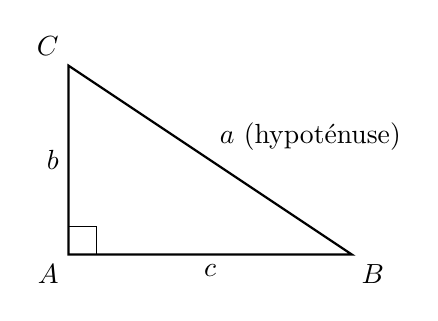
\begin{tikzpicture}[scale=1.2]
    % Triangle rectangle
    \coordinate (A) at (0,0);
    \coordinate (B) at (3,0);
    \coordinate (C) at (0,2);
    
    % Tracé du triangle
    \draw[thick] (A) -- (B) -- (C) -- cycle;
    
    % Angle droit
    \draw (0.3,0) -- (0.3,0.3) -- (0,0.3);
    
    % Étiquettes
    \node[below left] at (A) {$A$};
    \node[below right] at (B) {$B$};
    \node[above left] at (C) {$C$};
    
    % Côtés
    \node[below] at (1.5,0) {$c$};
    \node[left] at (0,1) {$b$};
    \node[above right] at (1.5,1) {$a$ (hypoténuse)};
\end{tikzpicture}
\end{center}

\subsection{Démonstration par la méthode des aires}

Considérons un carré de côté $(a + b)$ contenant quatre triangles rectangles identiques de côtés $a$, $b$ et d'hypoténuse $c$.

\begin{figure}[H]
\centering
\begin{minipage}{0.45\textwidth}
    \centering
    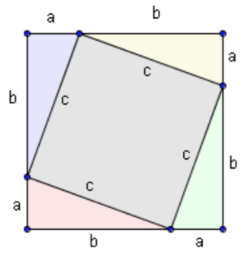
\includegraphics[width=0.8\textwidth]{chapitres/figures/chapitre_02_pythagore/fig_demo_pythagore_config_1.png}
    \caption{Configuration 1}
    \label{fig:config1}
\end{minipage}
\hfill
\begin{minipage}{0.45\textwidth}
    \centering
    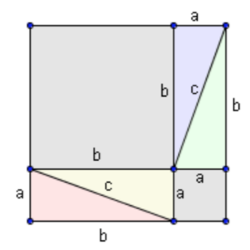
\includegraphics[width=0.8\textwidth]{chapitres/figures/chapitre_02_pythagore/fig_demo_pythagore_config_2.png}
    \caption{Configuration 2}
    \label{fig:config2}
\end{minipage}
\end{figure}

\textbf{Configuration 1 :} Aires = $(a+b)^2 = 4 \times \frac{ab}{2} + c^2 = 2ab + c^2$

\textbf{Configuration 2 :} Aires = $(a+b)^2 = 4 \times \frac{ab}{2} + a^2 + b^2 = 2ab + a^2 + b^2$

Comme l'aire est la même dans les deux configurations :
\[c^2 = a^2 + b^2\]

Ce qui démontre le théorème de Pythagore.

\section{Applications du théorème de Pythagore}

\subsection{Calculer la longueur de l'hypoténuse}

\begin{methode}{Calculer la longueur de l'hypoténuse}
Pour calculer la longueur de l'hypoténuse d'un triangle rectangle :
\begin{enumerate}
    \item Identifier le triangle rectangle et ses côtés
    \item Repérer l'hypoténuse (côté opposé à l'angle droit)
    \item Appliquer la formule : hypoténuse$^2$ = côté$_1^2$ + côté$_2^2$
    \item Calculer la racine carrée du résultat
\end{enumerate}
\end{methode}

\begin{exemple}
Un triangle $ABC$ est rectangle en $A$. $AB = 6$ cm et $AC = 8$ cm.\\
Calculer $BC$.

\textbf{Solution :}
\begin{itemize}
    \item Le triangle est rectangle en $A$, donc $BC$ est l'hypoténuse
    \item D'après le théorème de Pythagore : $BC^2 = AB^2 + AC^2$
    \item $BC^2 = 6^2 + 8^2 = 36 + 64 = 100$
    \item $BC = \sqrt{100} = 10$ cm
\end{itemize}
\end{exemple}

\subsection{Calculer la longueur d'un côté de l'angle droit}

\begin{methode}{Calculer la longueur d'un côté de l'angle droit}
Pour calculer la longueur d'un côté de l'angle droit :
\begin{enumerate}
    \item Identifier la longueur de l'hypoténuse et celle de l'autre côté de l'angle droit
    \item Appliquer la formule : hypoténuse$^2$ = côté$_1^2$ + côté$_2^2$
    \item Isoler le côté inconnu : côté$^2$ = hypoténuse$^2$ - autre côté$^2$
    \item Calculer la racine carrée du résultat
\end{enumerate}
\end{methode}

\begin{exemple}
Un triangle $DEF$ est rectangle en $D$. $DE = 5$ cm et $EF = 13$ cm.\\
Calculer $DF$.

\textbf{Solution :}
\begin{itemize}
    \item Le triangle est rectangle en $D$, donc $EF$ est l'hypoténuse
    \item D'après le théorème de Pythagore : $EF^2 = DE^2 + DF^2$
    \item $13^2 = 5^2 + DF^2$
    \item $169 = 25 + DF^2$
    \item $DF^2 = 169 - 25 = 144$
    \item $DF = \sqrt{144} = 12$ cm
\end{itemize}
\end{exemple}

\section{La réciproque du théorème de Pythagore}

\subsection{Énoncé de la réciproque}

\begin{propriete}{Réciproque du théorème de Pythagore}
Si, dans un triangle, le carré de la longueur du plus grand côté est égal à la somme des carrés des longueurs des deux autres côtés, alors ce triangle est rectangle.
\end{propriete}

\subsection{Utilisation de la réciproque}

\textbf{Objectif :} Déterminer si un triangle est rectangle en connaissant les longueurs de ses trois côtés.

\begin{methode}{Démontrer qu'un triangle est rectangle}
Pour démontrer qu'un triangle est rectangle :
\begin{enumerate}
    \item Identifier le plus grand côté du triangle
    \item Calculer le carré de sa longueur
    \item Calculer la somme des carrés des deux autres côtés
    \item Comparer les résultats :
    \begin{itemize}
        \item Si égalité : le triangle est rectangle
        \item Si inégalité : le triangle n'est pas rectangle
    \end{itemize}
\end{enumerate}
\end{methode}

\begin{exemple}
Un triangle a pour côtés 9 cm, 12 cm et 15 cm. Est-il rectangle ?

\textbf{Solution :}
\begin{itemize}
    \item Le plus grand côté mesure 15 cm
    \item $15^2 = 225$
    \item $9^2 + 12^2 = 81 + 144 = 225$
    \item Puisque $15^2 = 9^2 + 12^2$, le triangle est rectangle
    \item L'angle droit est opposé au côté de 15 cm
\end{itemize}
\end{exemple}

\begin{exemple}
Un triangle a pour côtés 7 cm, 8 cm et 10 cm. Est-il rectangle ?

\textbf{Solution :}
\begin{itemize}
    \item Le plus grand côté mesure 10 cm
    \item $10^2 = 100$
    \item $7^2 + 8^2 = 49 + 64 = 113$
    \item Puisque $100 \neq 113$, le triangle n'est pas rectangle
\end{itemize}
\end{exemple}

\section{Applications et résolution de problèmes}

\subsection{Problèmes de la vie courante}

\begin{exercice}{1 - L'échelle}
Une échelle de 4 m est appuyée contre un mur. Son pied est à 1,5 m du mur. À quelle hauteur le sommet de l'échelle touche-t-il le mur ?

\textbf{Solution :}
\begin{itemize}
    \item Triangle rectangle : mur, sol, échelle
    \item Hypoténuse : échelle = 4 m
    \item Un côté : distance au mur = 1,5 m
    \item Autre côté : hauteur = ?
\end{itemize}

$h^2 + 1,5^2 = 4^2$\\
$h^2 + 2,25 = 16$\\
$h^2 = 13,75$\\
$h = \sqrt{13,75} \approx 3,7$ m
\end{exercice}

\begin{exercice}{2 - Vérification d'équerrage}
Un maçon vérifie qu'un angle est droit en mesurant les côtés d'un triangle formé par deux murs et une diagonale. Il mesure : 3 m, 4 m et 5 m. L'angle est-il droit ?

\textbf{Solution :}
\begin{itemize}
    \item Plus grand côté : 5 m
    \item $5^2 = 25$
    \item $3^2 + 4^2 = 9 + 16 = 25$
    \item Égalité vérifiée $\Rightarrow$ l'angle est droit
\end{itemize}
\end{exercice}

\subsection{Utilisation de la calculatrice}

\textbf{Compétence :} Utiliser la touche $\sqrt{}$ (racine carrée) de la calculatrice.

\textbf{Exemple :} Calculer $\sqrt{75}$
\begin{itemize}
    \item $\sqrt{75} = \sqrt{25 \times 3} = \sqrt{25} \times \sqrt{3} = 5\sqrt{3} \approx 8,66$
\end{itemize}

\subsection{Calculs exacts et valeurs approchées}

\textbf{Calcul exact :} $\sqrt{50} = \sqrt{25 \times 2} = 5\sqrt{2}$ cm\\
\textbf{Valeur approchée :} $\sqrt{50} \approx 7,07$ cm (arrondi au centième)

\section{Théorème de Pythagore dans l'espace}

\subsection{Distance dans un pavé droit}

\textbf{Problème :} Calculer la longueur de la diagonale d'un pavé droit.

Pour un pavé droit de dimensions $a$, $b$ et $c$, la diagonale $d$ vérifie :
\[d^2 = a^2 + b^2 + c^2\]

\begin{exemple}
Pavé droit de dimensions 6 cm × 8 cm × 5 cm\\
$d^2 = 6^2 + 8^2 + 5^2 = 36 + 64 + 25 = 125$\\
$d = \sqrt{125} = 5\sqrt{5} \approx 11,18$ cm
\end{exemple}

\section{Compétences travaillées et automatismes}

\subsection{Compétences du socle commun}

\begin{itemize}
    \item \textbf{Chercher :} Identifier un triangle rectangle, choisir la bonne méthode
    \item \textbf{Modéliser :} Traduire un problème concret en calcul mathématique
    \item \textbf{Représenter :} Faire un schéma, coder une figure
    \item \textbf{Raisonner :} Justifier qu'un triangle est ou n'est pas rectangle
    \item \textbf{Calculer :} Effectuer des calculs avec des radicaux
    \item \textbf{Communiquer :} Rédiger une solution complète
\end{itemize}

\subsection{Automatismes à acquérir}

\begin{itemize}
    \item Reconnaître un triangle rectangle
    \item Identifier l'hypoténuse
    \item Appliquer le théorème direct ou sa réciproque
    \item Utiliser la calculatrice pour les racines carrées
    \item Connaître les "triplets pythagoriciens" usuels : (3;4;5), (5;12;13), (8;15;17)
\end{itemize}

\section{Exercices d'entraînement}

\subsection{Exercices de base}

\begin{exercice}{3}
Calculs directs :
\begin{enumerate}[label=\alph*)]
    \item Triangle rectangle : côtés 3 cm et 4 cm. Calculer l'hypoténuse.
    \item Triangle rectangle : hypoténuse 10 cm, un côté 6 cm. Calculer l'autre côté.
\end{enumerate}
\end{exercice}

\begin{exercice}{4}
Réciproque : Les triangles suivants sont-ils rectangles ?
\begin{enumerate}[label=\alph*)]
    \item Côtés : 7 cm, 24 cm, 25 cm
    \item Côtés : 6 cm, 7 cm, 8 cm
\end{enumerate}
\end{exercice}

\subsection{Exercices d'approfondissement}

\begin{exercice}{5}
\textbf{Problème du terrain}\\
Un terrain rectangulaire mesure 40 m sur 30 m. Calculer la longueur de sa diagonale.
\end{exercice}

\begin{exercice}{6}
\textbf{Navigation}\\
Un bateau part d'un port et navigue 12 km vers l'est puis 5 km vers le nord. À quelle distance se trouve-t-il du port ?
\end{exercice}

\begin{exercice}{7}
\textbf{Architecture}\\
Pour vérifier qu'un mur est perpendiculaire au sol, un architecte place un point A sur le mur à 3 m du sol, un point B au pied du mur, et un point C sur le sol à 4 m de B. Si AC = 5 m, le mur est-il perpendiculaire au sol ?
\end{exercice}

\section{Activité avec les TICE}

\subsection{Utilisation d'un logiciel de géométrie dynamique}

\textbf{Objectif :} Vérifier le théorème de Pythagore avec GeoGebra ou similaire

\textbf{Consignes :}
\begin{enumerate}
    \item Construire un triangle rectangle ABC
    \item Construire les carrés sur chaque côté
    \item Afficher les aires des trois carrés
    \item Modifier la forme du triangle et observer
    \item Conjecture sur la relation entre ces aires
\end{enumerate}

\section{Liens avec d'autres notions mathématiques}

\subsection{Distance entre deux points dans un repère}

Le théorème de Pythagore permet de calculer la distance entre deux points dans un repère orthonormé.

Si $A(x_A, y_A)$ et $B(x_B, y_B)$ sont deux points dans un repère orthonormé, alors la distance $AB$ est donnée par :
\[AB = \sqrt{(x_B - x_A)^2 + (y_B - y_A)^2}\]

\begin{exemple}
Calculons la distance entre les points $A(2, 3)$ et $B(6, 7)$ dans un repère orthonormé.

En appliquant le théorème de Pythagore :
\[AB^2 = (6-2)^2 + (7-3)^2 = 4^2 + 4^2 = 16 + 16 = 32\]
\[AB = \sqrt{32} = \sqrt{16 \times 2} = 4\sqrt{2}\]

La distance entre $A$ et $B$ est $4\sqrt{2}$ unités.
\end{exemple}

\subsection{Équations et théorème de Pythagore}

Le théorème de Pythagore conduit souvent à des équations qu'il faut résoudre pour trouver des longueurs.

\begin{exemple}
Dans un triangle rectangle $ABC$ rectangle en $A$, on sait que $AB = x$ cm, $AC = (x+3)$ cm et $BC = 17$ cm. Déterminons la valeur de $x$.

D'après le théorème de Pythagore :
\[BC^2 = AB^2 + AC^2\]
\[17^2 = x^2 + (x+3)^2\]
\[289 = x^2 + x^2 + 6x + 9\]
\[289 = 2x^2 + 6x + 9\]
\[2x^2 + 6x - 280 = 0\]
\[x^2 + 3x - 140 = 0\]

En factorisant : $(x - 10)(x + 14) = 0$

Les solutions sont $x = 10$ et $x = -14$.

Comme une longueur ne peut pas être négative, nous avons $x = 10$ cm.

Donc $AB = 10$ cm et $AC = 13$ cm.
\end{exemple}

\section{Pour aller plus loin}

\subsection{Histoire des mathématiques}
\begin{itemize}
    \item Les tablettes babyloniennes (Plimpton 322)
    \item La démonstration par le président Garfield
    \item Les différentes démonstrations du théorème (plus de 300 connues)
\end{itemize}

\subsection{Généralisation}
\begin{itemize}
    \item Théorème de Pythagore généralisé (loi des cosinus)
    \item Théorème de Pythagore dans l'espace à n dimensions
\end{itemize}

\subsection{Applications modernes}
\begin{itemize}
    \item GPS et géolocalisation
    \item Graphisme 3D et jeux vidéo
    \item Architecture et ingénierie
\end{itemize}

\section{Synthèse du chapitre}

\textbf{Ce qu'il faut retenir :}

\begin{enumerate}
    \item \textbf{Théorème de Pythagore :} Dans un triangle rectangle, hypoténuse$^2$ = côté$_1^2$ + côté$_2^2$
    \item \textbf{Réciproque :} Si dans un triangle, le carré du plus grand côté égale la somme des carrés des deux autres, alors le triangle est rectangle
    \item \textbf{Applications :} Calcul de longueurs, vérification d'angles droits, résolution de problèmes concrets
    \item \textbf{Méthodes :} Identification du triangle rectangle, application des formules, utilisation de la calculatrice
\end{enumerate}

\textbf{Liens avec d'autres chapitres :}
\begin{itemize}
    \item Racines carrées (chapitre précédent)
    \item Trigonométrie (chapitre à venir)
    \item Géométrie dans l'espace
    \item Fonctions (distance entre deux points dans un repère)
\end{itemize} 